% !TEX root = main.tex

\section{Decay-time Resoution}
\label{sec:Resolution}

The observed oscillation of B mesons is prone to dilution, if the detector resolution is of similar magnitude as the oscillation period. 
In the \Bs system, considering that the measured oscillation frequency of the \Bs \cite{PDG2014} and the average LHCb detector resolution \cite{LHCb-DP-2014-002} are both $\mathcal{O}(50 \fs^{-1})$, this is the case.
Therefore, it is crucial to correctly describe the decay time resolution in order to avoid a bias on the measurement of time dependent CP parameters. \newline
In the presented analysis, we assume a gaussian resolution function with different widths for each event. 
This gives rise to a per-event decay time error $\sigma_{t}$, which is computed separately for every event along with the proper time $t$, by the decay time fitter. 
Furthermore, the per-event decay time error $\sigma_{t}$ is usualy underestimated by the decay time fitter, 
making it necessary to derive a scaling function, which matches the per-event error to the actually measured decay time resolution. 
In the following, we investigate the Run1 and Run2 MC samples to find the proper decay time resolution in bins of the per-event decay time erros and derive a scaling function from that.      


\subsection{Formalism}

Describtion here ...




\subsection{Results}

Summary of results and MC/Data correction from $\Ds\kaon$ here ...


\begin{figure}[h]
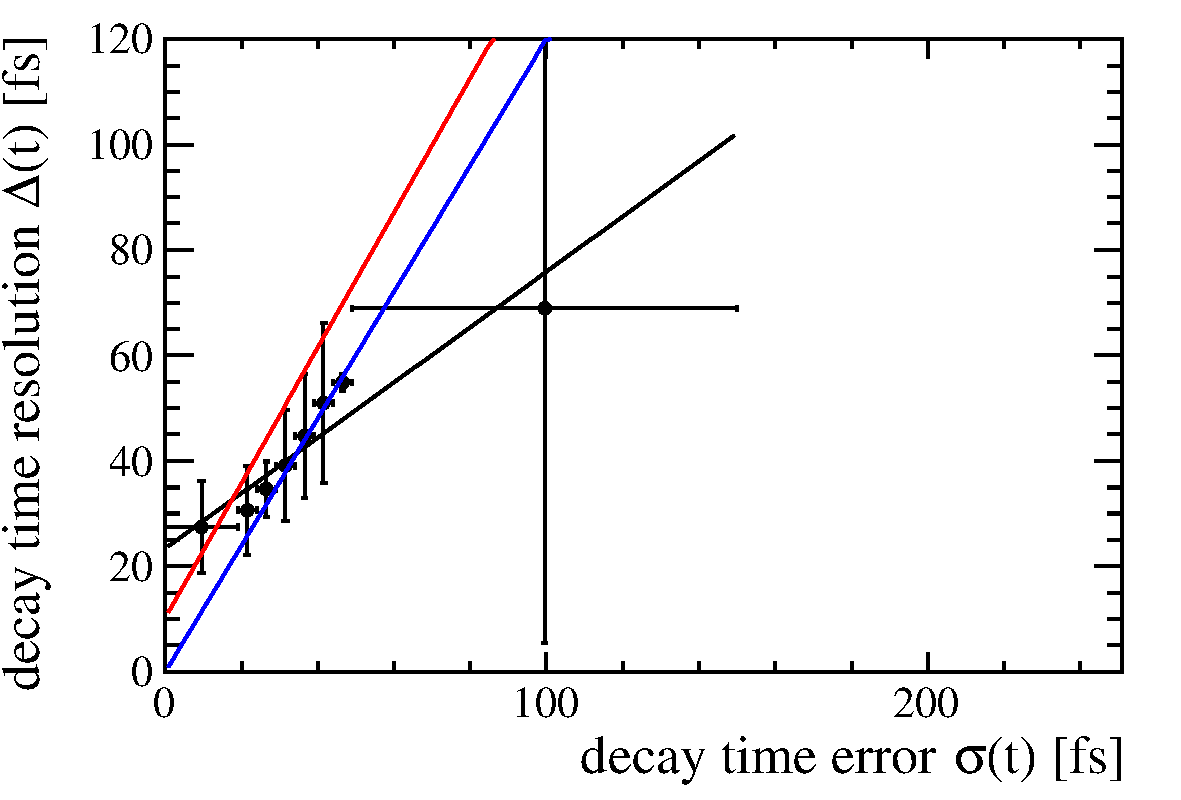
\includegraphics[height=7.4cm,width=0.7\textwidth]{figs/ProperTimeReso_MC.pdf}
\caption{Decay-time resolution of $\Bs\to\Ds\kaon\pion\pion$ candidates from MC. The fit described in the text is overlaid.}
\label{fig:ResoFit_compared}
\end{figure}


\begin{table}[h]
\centering
 \begin{tabular}{l || l l l | l l}
$\sigma_{t}$ Bin [fs] & $\sigma_{1}$ [fs] & $\sigma_{2}$ [fs] & $f_{1}$ & D & $\sigma_{eff}$ [fs] \\
\hline
0to19 & 22.57 $\pm$ 0.96 & 45.57 $\pm$ 4.061 & 0.827 $\pm$ 0.057 & 0.89 $\pm$ 0.067 & 27.46 $\pm$ 8.82 \\
19to24 & 24.64 $\pm$ 1.03 & 46.65 $\pm$ 3.109 & 0.768 $\pm$ 0.061 & 0.86 $\pm$ 0.070 & 30.64 $\pm$ 8.48 \\
24to29 & 30.96 $\pm$ 0.90 & 58.76 $\pm$ 5.684 & 0.884 $\pm$ 0.045 & 0.83 $\pm$ 0.05 & 34.66 $\pm$ 5.28 \\
29to34 & 35.28 $\pm$ 1.54 & 57 $\pm$ 6.698 & 0.839 $\pm$ 0.098 & 0.79 $\pm$ 0.10 & 39.09 $\pm$ 10.47 \\
34to39 & 37.05 $\pm$ 2.36 & 61.98 $\pm$ 5.769 & 0.707 $\pm$ 0.12 & 0.73 $\pm$ 0.12 & 44.76 $\pm$ 11.78 \\
39to44 & 68.38 $\pm$ 8.33 & 42.15 $\pm$ 3.583 & 0.331 $\pm$ 0.18 & 0.66 $\pm$ 0.16 & 50.98 $\pm$ 15.11 \\
44to49 & 199.9 $\pm$ 100.1 & 53.72 $\pm$ 1.419 & 0.020 $\pm$ 0.014 & 0.62 $\pm$ 0.02 & 54.89 $\pm$ 1.60 \\
49to150 & 68.75 $\pm$ 165.3 & 68.92 $\pm$ 4.603 & 0.001 $\pm$ 0.97 & 0.47 $\pm$ 0.65 & 68.92 $\pm$ 63.42 \\
\hline
\end{tabular}
\caption{Summary of the obtained parameters from the resolution fits described above.}
\label{table:ResoParams}
\end{table}

